\begin{figure}
  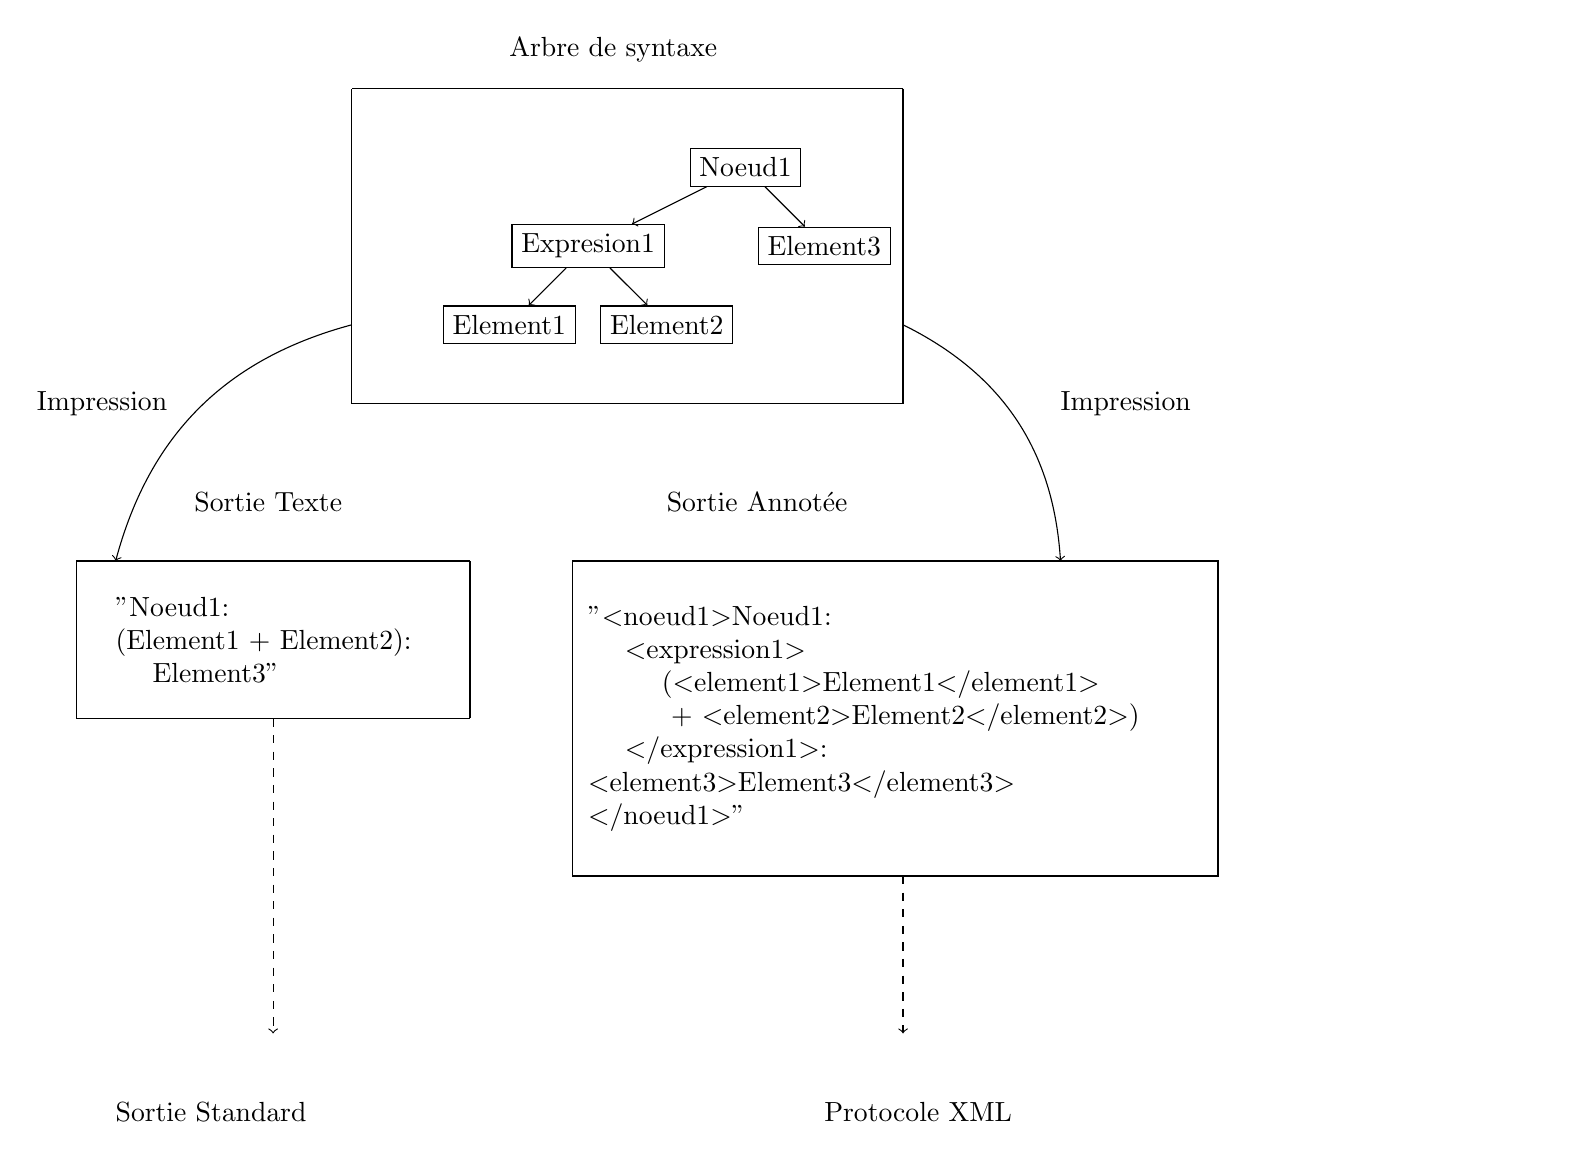
\begin{tikzpicture}
    %% Rectangle
    \draw (-2,-3) -- (-2,1);
    \draw (-2,-3) -- (5,-3);
    \draw (5,1) -- (-2,1);
    \draw (5,1) -- (5,-3);

    %% graphe1
    \node[text width=6cm] (titre1) at (3,1.5) {Arbre de syntaxe};
    \node[draw] (Noeud1) at (3,0) {Noeud1};
    \node[draw] (Expression1) at (1,-1) {Expresion1};
    \node[draw] (Element3) at (4,-1) {Element3};
    \node[draw] (Element1) at (0,-2) {Element1};
    \node[draw] (Element2) at (2,-2) {Element2};
    \draw[->] (Noeud1) -> (Expression1);
    \draw[->] (Noeud1) -> (Element3);
    \draw[->] (Expression1) -> (Element1);
    \draw[->] (Expression1) -> (Element2);

    %%print par défaut
    \draw (-5.5,-5) -- (-0.5,-5);
    \draw (-5.5,-5) -- (-5.5,-7);
    \draw (-5.5,-7) -- (-0.5,-7);
    \draw(-0.5,-5) -- (-0.5,-7);

    \node[text width=6cm] (titre3) at (-1,-4.25) {Sortie Texte};
    \node[text width=6cm] (Pp) at (-2,-6) {"Noeud1: \\ (Element1 + Element2):\\     ~~~~Element3"};


    \draw (0.8,-5) -- (0.8,-9) -- (9,-9) -- (9,-5) -- (0.8,-5);
    \node[text width=6cm] (titre3) at (5,-4.25) {Sortie Annotée};
    \node[text width=8cm] (Pp) at (5,-7) {
    "$\textless$noeud1$\textgreater$Noeud1: \\
     ~~~~$\textless$expression1$\textgreater$ \\
     ~~~~~~~~($\textless$element1$\textgreater$Element1$\textless$/element1$\textgreater$ \\
     ~~~~~~~~ + $\textless$element2$\textgreater$Element2$\textless$/element2$\textgreater$) \\
     ~~~~$\textless$/expression1$\textgreater$:
     ~~~~$\textless$element3$\textgreater$Element3$\textless$/element3$\textgreater$ \\
     $\textless$/noeud1$\textgreater$"};

    \node[text width=6cm] (plop) at (-3,-3) {Impression};
    \draw[->] (-2,-2) to [bend right] (-5,-5);

    \draw[->, dashed] (-3,-7) -- (-3,-11);
    \node[text width=6cm] (stdout) at (-2,-12) {Sortie Standard};

    \node[text width=6cm] (plop1) at (10,-3) {Impression};
    \draw[->] (5,-2) to [bend left] (7,-5);

    \draw[->, dashed] (5,-9) -- (5,-11);
    \node[text width=6cm] (stdout) at (7,-12) {Protocole XML};

  \end{tikzpicture}
  \caption{Traduction vers une mise en forme XML\label{xml}}
\end{figure}
